\documentclass[1p]{elsarticle_modified}
%\bibliographystyle{elsarticle-num}

%\usepackage[colorlinks]{hyperref}
%\usepackage{abbrmath_seonhwa} %\Abb, \Ascr, \Acal ,\Abf, \Afrak
\usepackage{amsfonts}
\usepackage{amssymb}
\usepackage{amsmath}
\usepackage{amsthm}
\usepackage{scalefnt}
\usepackage{amsbsy}
\usepackage{kotex}
\usepackage{caption}
\usepackage{subfig}
\usepackage{color}
\usepackage{graphicx}
\usepackage{xcolor} %% white, black, red, green, blue, cyan, magenta, yellow
\usepackage{float}
\usepackage{setspace}
\usepackage{hyperref}

\usepackage{tikz}
\usetikzlibrary{arrows}

\usepackage{multirow}
\usepackage{array} % fixed length table
\usepackage{hhline}

%%%%%%%%%%%%%%%%%%%%%
\makeatletter
\renewcommand*\env@matrix[1][\arraystretch]{%
	\edef\arraystretch{#1}%
	\hskip -\arraycolsep
	\let\@ifnextchar\new@ifnextchar
	\array{*\c@MaxMatrixCols c}}
\makeatother %https://tex.stackexchange.com/questions/14071/how-can-i-increase-the-line-spacing-in-a-matrix
%%%%%%%%%%%%%%%

\usepackage[normalem]{ulem}

\newcommand{\msout}[1]{\ifmmode\text{\sout{\ensuremath{#1}}}\else\sout{#1}\fi}
%SOURCE: \msout is \stkout macro in https://tex.stackexchange.com/questions/20609/strikeout-in-math-mode

\newcommand{\cancel}[1]{
	\ifmmode
	{\color{red}\msout{#1}}
	\else
	{\color{red}\sout{#1}}
	\fi
}

\newcommand{\add}[1]{
	{\color{blue}\uwave{#1}}
}

\newcommand{\replace}[2]{
	\ifmmode
	{\color{red}\msout{#1}}{\color{blue}\uwave{#2}}
	\else
	{\color{red}\sout{#1}}{\color{blue}\uwave{#2}}
	\fi
}

\newcommand{\Sol}{\mathcal{S}} %segment
\newcommand{\D}{D} %diagram
\newcommand{\A}{\mathcal{A}} %arc


%%%%%%%%%%%%%%%%%%%%%%%%%%%%%5 test

\def\sl{\operatorname{\textup{SL}}(2,\Cbb)}
\def\psl{\operatorname{\textup{PSL}}(2,\Cbb)}
\def\quan{\mkern 1mu \triangleright \mkern 1mu}

\theoremstyle{definition}
\newtheorem{thm}{Theorem}[section]
\newtheorem{prop}[thm]{Proposition}
\newtheorem{lem}[thm]{Lemma}
\newtheorem{ques}[thm]{Question}
\newtheorem{cor}[thm]{Corollary}
\newtheorem{defn}[thm]{Definition}
\newtheorem{exam}[thm]{Example}
\newtheorem{rmk}[thm]{Remark}
\newtheorem{alg}[thm]{Algorithm}

\newcommand{\I}{\sqrt{-1}}
\begin{document}

%\begin{frontmatter}
%
%\title{Boundary parabolic representations of knots up to 8 crossings}
%
%%% Group authors per affiliation:
%\author{Yunhi Cho} 
%\address{Department of Mathematics, University of Seoul, Seoul, Korea}
%\ead{yhcho@uos.ac.kr}
%
%
%\author{Seonhwa Kim} %\fnref{s_kim}}
%\address{Center for Geometry and Physics, Institute for Basic Science, Pohang, 37673, Korea}
%\ead{ryeona17@ibs.re.kr}
%
%\author{Hyuk Kim}
%\address{Department of Mathematical Sciences, Seoul National University, Seoul 08826, Korea}
%\ead{hyukkim@snu.ac.kr}
%
%\author{Seokbeom Yoon}
%\address{Department of Mathematical Sciences, Seoul National University, Seoul, 08826,  Korea}
%\ead{sbyoon15@snu.ac.kr}
%
%\begin{abstract}
%We find all boundary parabolic representation of knots up to 8 crossings.
%
%\end{abstract}
%\begin{keyword}
%    \MSC[2010] 57M25 
%\end{keyword}
%
%\end{frontmatter}

%\linenumbers
%\tableofcontents
%
\newcommand\colored[1]{\textcolor{white}{\rule[-0.35ex]{0.8em}{1.4ex}}\kern-0.8em\color{red} #1}%
%\newcommand\colored[1]{\textcolor{white}{ #1}\kern-2.17ex	\textcolor{white}{ #1}\kern-1.81ex	\textcolor{white}{ #1}\kern-2.15ex\color{red}#1	}

{\Large $\underline{12n_{0385}~(K12n_{0385})}$}

\setlength{\tabcolsep}{10pt}
\renewcommand{\arraystretch}{1.6}
\vspace{1cm}\begin{tabular}{m{100pt}>{\centering\arraybackslash}m{274pt}}
\multirow{5}{120pt}{
	\centering
	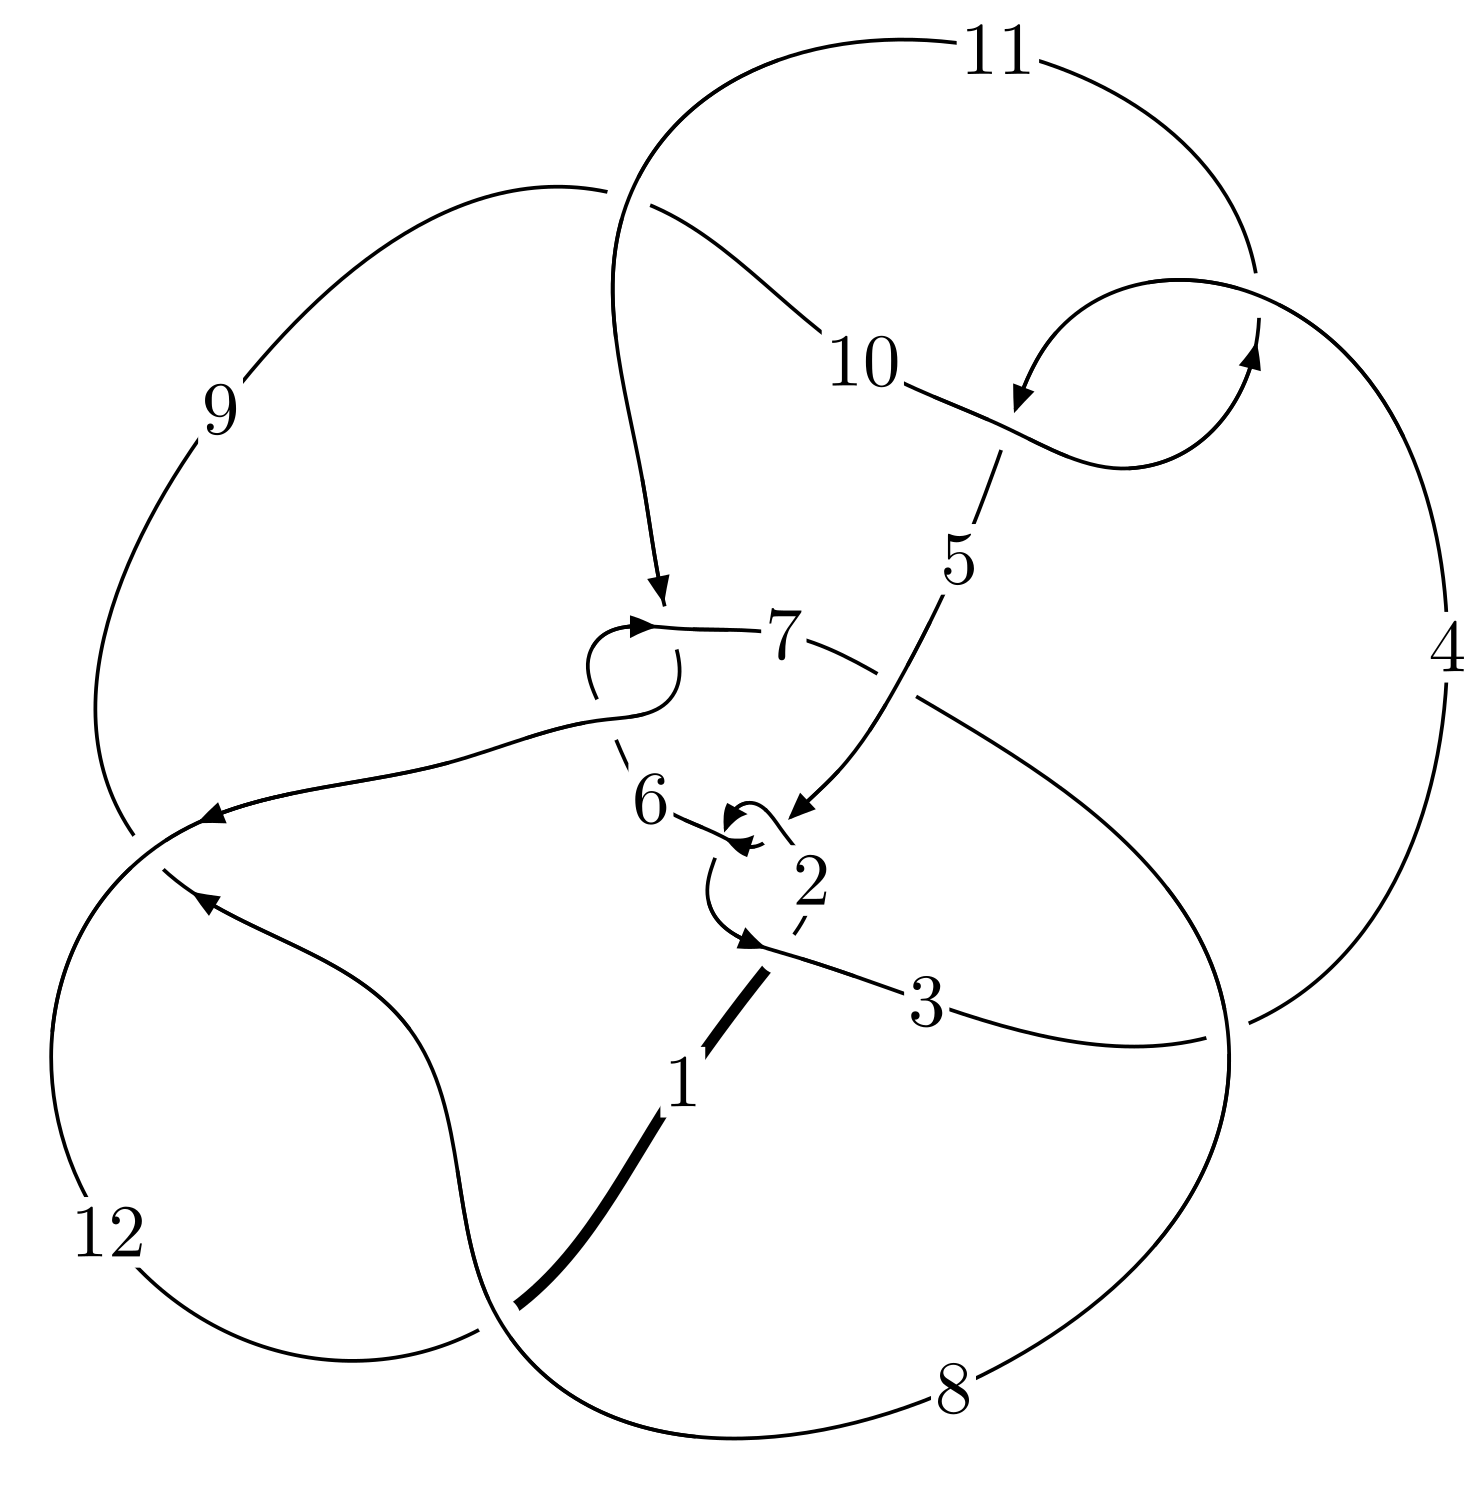
\includegraphics[width=112pt]{../../../GIT/diagram.site/Diagrams/png/2474_12n_0385.png}\\
\ \ \ A knot diagram\footnotemark}&
\allowdisplaybreaks
\textbf{Linearized knot diagam} \\
\cline{2-2}
 &
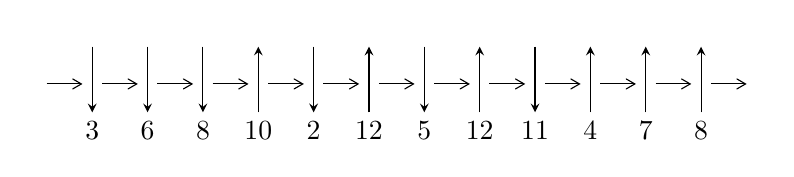
\begin{tikzpicture}[x=20pt, y=17pt]
	% nodes
	\node (C0) at (0, 0) {};
	\node (C1) at (1, 0) {};
	\node (C1U) at (1, +1) {};
	\node (C1D) at (1, -1) {3};

	\node (C2) at (2, 0) {};
	\node (C2U) at (2, +1) {};
	\node (C2D) at (2, -1) {6};

	\node (C3) at (3, 0) {};
	\node (C3U) at (3, +1) {};
	\node (C3D) at (3, -1) {8};

	\node (C4) at (4, 0) {};
	\node (C4U) at (4, +1) {};
	\node (C4D) at (4, -1) {10};

	\node (C5) at (5, 0) {};
	\node (C5U) at (5, +1) {};
	\node (C5D) at (5, -1) {2};

	\node (C6) at (6, 0) {};
	\node (C6U) at (6, +1) {};
	\node (C6D) at (6, -1) {12};

	\node (C7) at (7, 0) {};
	\node (C7U) at (7, +1) {};
	\node (C7D) at (7, -1) {5};

	\node (C8) at (8, 0) {};
	\node (C8U) at (8, +1) {};
	\node (C8D) at (8, -1) {12};

	\node (C9) at (9, 0) {};
	\node (C9U) at (9, +1) {};
	\node (C9D) at (9, -1) {11};

	\node (C10) at (10, 0) {};
	\node (C10U) at (10, +1) {};
	\node (C10D) at (10, -1) {4};

	\node (C11) at (11, 0) {};
	\node (C11U) at (11, +1) {};
	\node (C11D) at (11, -1) {7};

	\node (C12) at (12, 0) {};
	\node (C12U) at (12, +1) {};
	\node (C12D) at (12, -1) {8};
	\node (C13) at (13, 0) {};

	% arrows
	\draw[->,>={angle 60}]
	(C0) edge (C1) (C1) edge (C2) (C2) edge (C3) (C3) edge (C4) (C4) edge (C5) (C5) edge (C6) (C6) edge (C7) (C7) edge (C8) (C8) edge (C9) (C9) edge (C10) (C10) edge (C11) (C11) edge (C12) (C12) edge (C13) ;	\draw[->,>=stealth]
	(C1U) edge (C1D) (C2U) edge (C2D) (C3U) edge (C3D) (C4D) edge (C4U) (C5U) edge (C5D) (C6D) edge (C6U) (C7U) edge (C7D) (C8D) edge (C8U) (C9U) edge (C9D) (C10D) edge (C10U) (C11D) edge (C11U) (C12D) edge (C12U) ;
	\end{tikzpicture} \\
\hhline{~~} \\& 
\textbf{Solving Sequence} \\ \cline{2-2} 
 &
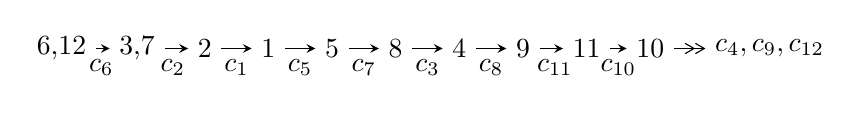
\begin{tikzpicture}[x=23pt, y=7pt]
	% node
	\node (A0) at (-1/8, 0) {6,12};
	\node (A1) at (17/16, 0) {3,7};
	\node (A2) at (17/8, 0) {2};
	\node (A3) at (25/8, 0) {1};
	\node (A4) at (33/8, 0) {5};
	\node (A5) at (41/8, 0) {8};
	\node (A6) at (49/8, 0) {4};
	\node (A7) at (57/8, 0) {9};
	\node (A8) at (65/8, 0) {11};
	\node (A9) at (73/8, 0) {10};
	\node (C1) at (1/2, -1) {$c_{6}$};
	\node (C2) at (13/8, -1) {$c_{2}$};
	\node (C3) at (21/8, -1) {$c_{1}$};
	\node (C4) at (29/8, -1) {$c_{5}$};
	\node (C5) at (37/8, -1) {$c_{7}$};
	\node (C6) at (45/8, -1) {$c_{3}$};
	\node (C7) at (53/8, -1) {$c_{8}$};
	\node (C8) at (61/8, -1) {$c_{11}$};
	\node (C9) at (69/8, -1) {$c_{10}$};
	\node (A10) at (11, 0) {$c_{4},c_{9},c_{12}$};

	% edge
	\draw[->,>=stealth]	
	(A0) edge (A1) (A1) edge (A2) (A2) edge (A3) (A3) edge (A4) (A4) edge (A5) (A5) edge (A6) (A6) edge (A7) (A7) edge (A8) (A8) edge (A9) ;
	\draw[->>,>={angle 60}]	
	(A9) edge (A10);
\end{tikzpicture} \\ 

\end{tabular} \\

\footnotetext{
The image of knot diagram is generated by the software ``\textbf{Draw programme}" developed by Andrew Bartholomew(\url{http://www.layer8.co.uk/maths/draw/index.htm\#Running-draw}), where we modified some parts for our purpose(\url{https://github.com/CATsTAILs/LinksPainter}).
}\phantom \\ \newline 
\centering \textbf{Ideals for irreducible components\footnotemark of $X_{\text{par}}$} 
 
\begin{align*}
I^u_{1}&=\langle 
-2.29531\times10^{124} u^{55}-5.17327\times10^{124} u^{54}+\cdots+4.70448\times10^{122} b+9.01469\times10^{124},\\
\phantom{I^u_{1}}&\phantom{= \langle  }7.90126\times10^{124} u^{55}+1.78040\times10^{125} u^{54}+\cdots+4.70448\times10^{122} a-3.09074\times10^{125},\;u^{56}+2 u^{55}+\cdots-15 u+1\rangle \\
I^u_{2}&=\langle 
126249067 u^{19}-438214333 u^{18}+\cdots+593361451 b+602467017,\\
\phantom{I^u_{2}}&\phantom{= \langle  }-1023562993 u^{19}+1683425057 u^{18}+\cdots+593361451 a+2283136733,\;u^{20}- u^{19}+\cdots- u+1\rangle \\
\\
\end{align*}
\raggedright * 2 irreducible components of $\dim_{\mathbb{C}}=0$, with total 76 representations.\\
\footnotetext{All coefficients of polynomials are rational numbers. But the coefficients are sometimes approximated in decimal forms when there is not enough margin.}
\newpage
\renewcommand{\arraystretch}{1}
\centering \section*{I. $I^u_{1}= \langle -2.30\times10^{124} u^{55}-5.17\times10^{124} u^{54}+\cdots+4.70\times10^{122} b+9.01\times10^{124},\;7.90\times10^{124} u^{55}+1.78\times10^{125} u^{54}+\cdots+4.70\times10^{122} a-3.09\times10^{125},\;u^{56}+2 u^{55}+\cdots-15 u+1 \rangle$}
\flushleft \textbf{(i) Arc colorings}\\
\begin{tabular}{m{7pt} m{180pt} m{7pt} m{180pt} }
\flushright $a_{6}=$&$\begin{pmatrix}1\\0\end{pmatrix}$ \\
\flushright $a_{12}=$&$\begin{pmatrix}0\\u\end{pmatrix}$ \\
\flushright $a_{3}=$&$\begin{pmatrix}-167.952 u^{55}-378.447 u^{54}+\cdots-7319.21 u+656.977\\48.7899 u^{55}+109.965 u^{54}+\cdots+2128.78 u-191.619\end{pmatrix}$ \\
\flushright $a_{7}=$&$\begin{pmatrix}1\\- u^2\end{pmatrix}$ \\
\flushright $a_{2}=$&$\begin{pmatrix}-119.162 u^{55}-268.482 u^{54}+\cdots-5190.43 u+465.357\\48.7899 u^{55}+109.965 u^{54}+\cdots+2128.78 u-191.619\end{pmatrix}$ \\
\flushright $a_{1}=$&$\begin{pmatrix}50.7952 u^{55}+115.863 u^{54}+\cdots+2093.41 u-184.274\\-35.5785 u^{55}-80.8855 u^{54}+\cdots-1476.67 u+130.375\end{pmatrix}$ \\
\flushright $a_{5}=$&$\begin{pmatrix}-145.156 u^{55}-329.196 u^{54}+\cdots-6101.43 u+545.139\\87.4444 u^{55}+197.890 u^{54}+\cdots+3716.70 u-332.270\end{pmatrix}$ \\
\flushright $a_{8}=$&$\begin{pmatrix}21.0734 u^{55}+49.2382 u^{54}+\cdots+731.326 u-59.8342\\-19.6677 u^{55}-45.0556 u^{54}+\cdots-774.695 u+66.8772\end{pmatrix}$ \\
\flushright $a_{4}=$&$\begin{pmatrix}332.270 u^{55}+751.984 u^{54}+\cdots+14152.1 u-1267.35\\-185.312 u^{55}-419.091 u^{54}+\cdots-7917.98 u+708.943\end{pmatrix}$ \\
\flushright $a_{9}=$&$\begin{pmatrix}21.0734 u^{55}+49.2382 u^{54}+\cdots+731.326 u-59.8342\\-21.9298 u^{55}-50.2637 u^{54}+\cdots-859.993 u+73.9686\end{pmatrix}$ \\
\flushright $a_{11}=$&$\begin{pmatrix}- u\\u^3+u\end{pmatrix}$ \\
\flushright $a_{10}=$&$\begin{pmatrix}20.4358 u^{55}+47.7320 u^{54}+\cdots+712.161 u-58.4629\\-21.2114 u^{55}-48.5599 u^{54}+\cdots-838.002 u+72.3663\end{pmatrix}$\\&\end{tabular}
\flushleft \textbf{(ii) Obstruction class $= -1$}\\~\\
\flushleft \textbf{(iii) Cusp Shapes $= -217.435 u^{55}-492.105 u^{54}+\cdots-9258.95 u+822.622$}\\~\\
\newpage\renewcommand{\arraystretch}{1}
\flushleft \textbf{(iv) u-Polynomials at the component}\newline \\
\begin{tabular}{m{50pt}|m{274pt}}
Crossings & \hspace{64pt}u-Polynomials at each crossing \\
\hline $$\begin{aligned}c_{1}\end{aligned}$$&$\begin{aligned}
&u^{56}+13 u^{55}+\cdots+u+1
\end{aligned}$\\
\hline $$\begin{aligned}c_{2},c_{5}\end{aligned}$$&$\begin{aligned}
&u^{56}+3 u^{55}+\cdots-7 u+1
\end{aligned}$\\
\hline $$\begin{aligned}c_{3}\end{aligned}$$&$\begin{aligned}
&u^{56}+2 u^{55}+\cdots+43738 u+6847
\end{aligned}$\\
\hline $$\begin{aligned}c_{4},c_{10}\end{aligned}$$&$\begin{aligned}
&u^{56}+u^{55}+\cdots+130 u+43
\end{aligned}$\\
\hline $$\begin{aligned}c_{6},c_{11}\end{aligned}$$&$\begin{aligned}
&u^{56}-2 u^{55}+\cdots+15 u+1
\end{aligned}$\\
\hline $$\begin{aligned}c_{7}\end{aligned}$$&$\begin{aligned}
&u^{56}+u^{55}+\cdots-8 u+19
\end{aligned}$\\
\hline $$\begin{aligned}c_{8},c_{12}\end{aligned}$$&$\begin{aligned}
&u^{56}+8 u^{55}+\cdots+25217681 u+3589991
\end{aligned}$\\
\hline $$\begin{aligned}c_{9}\end{aligned}$$&$\begin{aligned}
&u^{56}+21 u^{55}+\cdots+36162 u+1849
\end{aligned}$\\
\hline
\end{tabular}\\~\\
\newpage\renewcommand{\arraystretch}{1}
\flushleft \textbf{(v) Riley Polynomials at the component}\newline \\
\begin{tabular}{m{50pt}|m{274pt}}
Crossings & \hspace{64pt}Riley Polynomials at each crossing \\
\hline $$\begin{aligned}c_{1}\end{aligned}$$&$\begin{aligned}
&y^{56}+67 y^{55}+\cdots-305 y+1
\end{aligned}$\\
\hline $$\begin{aligned}c_{2},c_{5}\end{aligned}$$&$\begin{aligned}
&y^{56}-13 y^{55}+\cdots- y+1
\end{aligned}$\\
\hline $$\begin{aligned}c_{3}\end{aligned}$$&$\begin{aligned}
&y^{56}+76 y^{55}+\cdots+2879627170 y+46881409
\end{aligned}$\\
\hline $$\begin{aligned}c_{4},c_{10}\end{aligned}$$&$\begin{aligned}
&y^{56}+21 y^{55}+\cdots+36162 y+1849
\end{aligned}$\\
\hline $$\begin{aligned}c_{6},c_{11}\end{aligned}$$&$\begin{aligned}
&y^{56}+6 y^{55}+\cdots-25 y+1
\end{aligned}$\\
\hline $$\begin{aligned}c_{7}\end{aligned}$$&$\begin{aligned}
&y^{56}-9 y^{55}+\cdots+17302 y+361
\end{aligned}$\\
\hline $$\begin{aligned}c_{8},c_{12}\end{aligned}$$&$\begin{aligned}
&y^{56}-78 y^{55}+\cdots+166741384065503 y+12888035380081
\end{aligned}$\\
\hline $$\begin{aligned}c_{9}\end{aligned}$$&$\begin{aligned}
&y^{56}+49 y^{55}+\cdots-27712598 y+3418801
\end{aligned}$\\
\hline
\end{tabular}\\~\\
\newpage\flushleft \textbf{(vi) Complex Volumes and Cusp Shapes}
$$\begin{array}{c|c|c}  
\text{Solutions to }I^u_{1}& \I (\text{vol} + \sqrt{-1}CS) & \text{Cusp shape}\\
 \hline 
\begin{aligned}
u &= \phantom{-}0.662954 + 0.763312 I \\
a &= \phantom{-}0.109755 + 0.857727 I \\
b &= \phantom{-}0.710096 - 0.628504 I\end{aligned}
 & -0.01661 + 7.26026 I & \phantom{-0.000000 } 0. - 10.22253 I \\ \hline\begin{aligned}
u &= \phantom{-}0.662954 - 0.763312 I \\
a &= \phantom{-}0.109755 - 0.857727 I \\
b &= \phantom{-}0.710096 + 0.628504 I\end{aligned}
 & -0.01661 - 7.26026 I & \phantom{-0.000000 -}0. + 10.22253 I \\ \hline\begin{aligned}
u &= -0.666863 + 0.770647 I \\
a &= \phantom{-}0.887690 - 0.725522 I \\
b &= -0.221964 + 0.922686 I\end{aligned}
 & \phantom{-}1.78699 - 2.38449 I & \phantom{-0.000000 } 0 \\ \hline\begin{aligned}
u &= -0.666863 - 0.770647 I \\
a &= \phantom{-}0.887690 + 0.725522 I \\
b &= -0.221964 - 0.922686 I\end{aligned}
 & \phantom{-}1.78699 + 2.38449 I & \phantom{-0.000000 } 0 \\ \hline\begin{aligned}
u &= \phantom{-}0.865491 + 0.431238 I \\
a &= \phantom{-}0.37766 - 3.20632 I \\
b &= -0.415607 + 0.220395 I\end{aligned}
 & -1.50834 + 5.13908 I & -1.64354 - 9.78620 I \\ \hline\begin{aligned}
u &= \phantom{-}0.865491 - 0.431238 I \\
a &= \phantom{-}0.37766 + 3.20632 I \\
b &= -0.415607 - 0.220395 I\end{aligned}
 & -1.50834 - 5.13908 I & -1.64354 + 9.78620 I \\ \hline\begin{aligned}
u &= -0.694616 + 0.641622 I \\
a &= -0.163620 + 0.995740 I \\
b &= -0.598031 - 0.619979 I\end{aligned}
 & \phantom{-}2.04092 - 2.37552 I & \phantom{-}3.14853 + 4.55601 I \\ \hline\begin{aligned}
u &= -0.694616 - 0.641622 I \\
a &= -0.163620 - 0.995740 I \\
b &= -0.598031 + 0.619979 I\end{aligned}
 & \phantom{-}2.04092 + 2.37552 I & \phantom{-}3.14853 - 4.55601 I \\ \hline\begin{aligned}
u &= \phantom{-}0.888013 + 0.699797 I \\
a &= \phantom{-}0.138881 - 0.344888 I \\
b &= \phantom{-}0.838168 + 0.413727 I\end{aligned}
 & -0.60327 + 3.12252 I & \phantom{-0.000000 } 0 \\ \hline\begin{aligned}
u &= \phantom{-}0.888013 - 0.699797 I \\
a &= \phantom{-}0.138881 + 0.344888 I \\
b &= \phantom{-}0.838168 - 0.413727 I\end{aligned}
 & -0.60327 - 3.12252 I & \phantom{-0.000000 } 0\\
 \hline 
 \end{array}$$\newpage$$\begin{array}{c|c|c}  
\text{Solutions to }I^u_{1}& \I (\text{vol} + \sqrt{-1}CS) & \text{Cusp shape}\\
 \hline 
\begin{aligned}
u &= \phantom{-}0.190436 + 1.123830 I \\
a &= \phantom{-}0.444310 + 0.527604 I \\
b &= -0.365972 + 0.069044 I\end{aligned}
 & -4.50386 - 1.21393 I & \phantom{-0.000000 } 0 \\ \hline\begin{aligned}
u &= \phantom{-}0.190436 - 1.123830 I \\
a &= \phantom{-}0.444310 - 0.527604 I \\
b &= -0.365972 - 0.069044 I\end{aligned}
 & -4.50386 + 1.21393 I & \phantom{-0.000000 } 0 \\ \hline\begin{aligned}
u &= -0.855002 + 0.041630 I \\
a &= -1.26036 + 1.03025 I \\
b &= -0.064318 - 0.244656 I\end{aligned}
 & \phantom{-}1.51091 - 0.09931 I & \phantom{-}7.48576 - 0.57256 I \\ \hline\begin{aligned}
u &= -0.855002 - 0.041630 I \\
a &= -1.26036 - 1.03025 I \\
b &= -0.064318 + 0.244656 I\end{aligned}
 & \phantom{-}1.51091 + 0.09931 I & \phantom{-}7.48576 + 0.57256 I \\ \hline\begin{aligned}
u &= -1.154250 + 0.028922 I \\
a &= -0.67805 + 1.69251 I \\
b &= \phantom{-}0.898070 - 0.760890 I\end{aligned}
 & \phantom{-}4.21997 + 2.88917 I & \phantom{-0.000000 } 0 \\ \hline\begin{aligned}
u &= -1.154250 - 0.028922 I \\
a &= -0.67805 - 1.69251 I \\
b &= \phantom{-}0.898070 + 0.760890 I\end{aligned}
 & \phantom{-}4.21997 - 2.88917 I & \phantom{-0.000000 } 0 \\ \hline\begin{aligned}
u &= \phantom{-}0.298553 + 0.783068 I \\
a &= \phantom{-}1.47696 + 1.31436 I \\
b &= \phantom{-}1.216760 - 0.521960 I\end{aligned}
 & -1.71963 + 1.34220 I & \phantom{-}1.33019 - 5.27887 I \\ \hline\begin{aligned}
u &= \phantom{-}0.298553 - 0.783068 I \\
a &= \phantom{-}1.47696 - 1.31436 I \\
b &= \phantom{-}1.216760 + 0.521960 I\end{aligned}
 & -1.71963 - 1.34220 I & \phantom{-}1.33019 + 5.27887 I \\ \hline\begin{aligned}
u &= \phantom{-}0.236859 + 1.215390 I \\
a &= -0.760833 - 0.660762 I \\
b &= \phantom{-}0.479782 + 0.683588 I\end{aligned}
 & -3.22157 - 1.15649 I & \phantom{-0.000000 } 0 \\ \hline\begin{aligned}
u &= \phantom{-}0.236859 - 1.215390 I \\
a &= -0.760833 + 0.660762 I \\
b &= \phantom{-}0.479782 - 0.683588 I\end{aligned}
 & -3.22157 + 1.15649 I & \phantom{-0.000000 } 0\\
 \hline 
 \end{array}$$\newpage$$\begin{array}{c|c|c}  
\text{Solutions to }I^u_{1}& \I (\text{vol} + \sqrt{-1}CS) & \text{Cusp shape}\\
 \hline 
\begin{aligned}
u &= -1.221310 + 0.412682 I \\
a &= \phantom{-}0.141595 - 0.224601 I \\
b &= -0.965402 + 0.220051 I\end{aligned}
 & \phantom{-}0.709733 + 0.991277 I & \phantom{-0.000000 } 0 \\ \hline\begin{aligned}
u &= -1.221310 - 0.412682 I \\
a &= \phantom{-}0.141595 + 0.224601 I \\
b &= -0.965402 - 0.220051 I\end{aligned}
 & \phantom{-}0.709733 - 0.991277 I & \phantom{-0.000000 } 0 \\ \hline\begin{aligned}
u &= \phantom{-}0.681846 + 0.011526 I \\
a &= -3.05207 - 2.44743 I \\
b &= \phantom{-}0.446392 + 0.849165 I\end{aligned}
 & \phantom{-}1.13214 - 4.01858 I & \phantom{-}5.94853 + 4.16003 I \\ \hline\begin{aligned}
u &= \phantom{-}0.681846 - 0.011526 I \\
a &= -3.05207 + 2.44743 I \\
b &= \phantom{-}0.446392 - 0.849165 I\end{aligned}
 & \phantom{-}1.13214 + 4.01858 I & \phantom{-}5.94853 - 4.16003 I \\ \hline\begin{aligned}
u &= \phantom{-}0.529724 + 0.424634 I \\
a &= \phantom{-}0.48742 + 1.49607 I \\
b &= -0.811392 + 0.067619 I\end{aligned}
 & -3.17521 + 4.65332 I & -7.74651 - 6.05847 I \\ \hline\begin{aligned}
u &= \phantom{-}0.529724 - 0.424634 I \\
a &= \phantom{-}0.48742 - 1.49607 I \\
b &= -0.811392 - 0.067619 I\end{aligned}
 & -3.17521 - 4.65332 I & -7.74651 + 6.05847 I \\ \hline\begin{aligned}
u &= -0.153495 + 1.312610 I \\
a &= -1.18611 + 0.82511 I \\
b &= -0.994161 - 0.290702 I\end{aligned}
 & -6.82465 - 2.95148 I & \phantom{-0.000000 } 0 \\ \hline\begin{aligned}
u &= -0.153495 - 1.312610 I \\
a &= -1.18611 - 0.82511 I \\
b &= -0.994161 + 0.290702 I\end{aligned}
 & -6.82465 + 2.95148 I & \phantom{-0.000000 } 0 \\ \hline\begin{aligned}
u &= \phantom{-}1.054190 + 0.817175 I \\
a &= \phantom{-}1.74185 + 1.23072 I \\
b &= -0.915264 - 1.067760 I\end{aligned}
 & \phantom{-}10.62210 + 1.04027 I & \phantom{-0.000000 } 0 \\ \hline\begin{aligned}
u &= \phantom{-}1.054190 - 0.817175 I \\
a &= \phantom{-}1.74185 - 1.23072 I \\
b &= -0.915264 + 1.067760 I\end{aligned}
 & \phantom{-}10.62210 - 1.04027 I & \phantom{-0.000000 } 0\\
 \hline 
 \end{array}$$\newpage$$\begin{array}{c|c|c}  
\text{Solutions to }I^u_{1}& \I (\text{vol} + \sqrt{-1}CS) & \text{Cusp shape}\\
 \hline 
\begin{aligned}
u &= -0.716286 + 1.170940 I \\
a &= -0.257562 + 1.315470 I \\
b &= -1.281030 - 0.421786 I\end{aligned}
 & -1.88294 - 7.50272 I & \phantom{-0.000000 } 0 \\ \hline\begin{aligned}
u &= -0.716286 - 1.170940 I \\
a &= -0.257562 - 1.315470 I \\
b &= -1.281030 + 0.421786 I\end{aligned}
 & -1.88294 + 7.50272 I & \phantom{-0.000000 } 0 \\ \hline\begin{aligned}
u &= \phantom{-}1.085940 + 0.879913 I \\
a &= \phantom{-}0.23842 - 2.61162 I \\
b &= -1.07014 + 0.95854 I\end{aligned}
 & \phantom{-}10.09000 + 8.41326 I & \phantom{-0.000000 } 0 \\ \hline\begin{aligned}
u &= \phantom{-}1.085940 - 0.879913 I \\
a &= \phantom{-}0.23842 + 2.61162 I \\
b &= -1.07014 - 0.95854 I\end{aligned}
 & \phantom{-}10.09000 - 8.41326 I & \phantom{-0.000000 } 0 \\ \hline\begin{aligned}
u &= \phantom{-}0.87694 + 1.16695 I \\
a &= \phantom{-}0.46590 - 1.84575 I \\
b &= -0.910716 + 0.995484 I\end{aligned}
 & \phantom{-}9.48260 + 6.10181 I & \phantom{-0.000000 } 0 \\ \hline\begin{aligned}
u &= \phantom{-}0.87694 - 1.16695 I \\
a &= \phantom{-}0.46590 + 1.84575 I \\
b &= -0.910716 - 0.995484 I\end{aligned}
 & \phantom{-}9.48260 - 6.10181 I & \phantom{-0.000000 } 0 \\ \hline\begin{aligned}
u &= -0.201309 + 0.484082 I \\
a &= \phantom{-}5.17876 - 2.75312 I \\
b &= \phantom{-}0.764547 + 1.016520 I\end{aligned}
 & \phantom{-}0.36376 - 4.79110 I & -12.4271 + 7.9106 I \\ \hline\begin{aligned}
u &= -0.201309 - 0.484082 I \\
a &= \phantom{-}5.17876 + 2.75312 I \\
b &= \phantom{-}0.764547 - 1.016520 I\end{aligned}
 & \phantom{-}0.36376 + 4.79110 I & -12.4271 - 7.9106 I \\ \hline\begin{aligned}
u &= \phantom{-}0.41214 + 1.42834 I \\
a &= \phantom{-}0.36344 + 1.45804 I \\
b &= \phantom{-}1.088950 - 0.558550 I\end{aligned}
 & -5.09935 + 3.68934 I & \phantom{-0.000000 } 0 \\ \hline\begin{aligned}
u &= \phantom{-}0.41214 - 1.42834 I \\
a &= \phantom{-}0.36344 - 1.45804 I \\
b &= \phantom{-}1.088950 + 0.558550 I\end{aligned}
 & -5.09935 - 3.68934 I & \phantom{-0.000000 } 0\\
 \hline 
 \end{array}$$\newpage$$\begin{array}{c|c|c}  
\text{Solutions to }I^u_{1}& \I (\text{vol} + \sqrt{-1}CS) & \text{Cusp shape}\\
 \hline 
\begin{aligned}
u &= \phantom{-}0.92562 + 1.19150 I \\
a &= \phantom{-}0.86660 + 1.42318 I \\
b &= -1.030690 - 0.930366 I\end{aligned}
 & \phantom{-}9.09077 - 0.96024 I & \phantom{-0.000000 } 0 \\ \hline\begin{aligned}
u &= \phantom{-}0.92562 - 1.19150 I \\
a &= \phantom{-}0.86660 - 1.42318 I \\
b &= -1.030690 + 0.930366 I\end{aligned}
 & \phantom{-}9.09077 + 0.96024 I & \phantom{-0.000000 } 0 \\ \hline\begin{aligned}
u &= \phantom{-}0.107311 + 0.465903 I \\
a &= \phantom{-}0.942601 + 0.990213 I \\
b &= \phantom{-}0.847141 - 0.344738 I\end{aligned}
 & -1.82336 + 0.66526 I & -4.71538 - 3.25851 I \\ \hline\begin{aligned}
u &= \phantom{-}0.107311 - 0.465903 I \\
a &= \phantom{-}0.942601 - 0.990213 I \\
b &= \phantom{-}0.847141 + 0.344738 I\end{aligned}
 & -1.82336 - 0.66526 I & -4.71538 + 3.25851 I \\ \hline\begin{aligned}
u &= -1.06310 + 1.14192 I \\
a &= -1.29601 + 1.16872 I \\
b &= \phantom{-}0.831104 - 1.076510 I\end{aligned}
 & \phantom{-}9.09155 - 8.12513 I & \phantom{-0.000000 } 0 \\ \hline\begin{aligned}
u &= -1.06310 - 1.14192 I \\
a &= -1.29601 - 1.16872 I \\
b &= \phantom{-}0.831104 + 1.076510 I\end{aligned}
 & \phantom{-}9.09155 + 8.12513 I & \phantom{-0.000000 } 0 \\ \hline\begin{aligned}
u &= -1.20609 + 1.00543 I \\
a &= -0.48936 - 1.88232 I \\
b &= \phantom{-}0.819158 + 1.011510 I\end{aligned}
 & \phantom{-}9.61530 - 0.06348 I & \phantom{-0.000000 } 0 \\ \hline\begin{aligned}
u &= -1.20609 - 1.00543 I \\
a &= -0.48936 + 1.88232 I \\
b &= \phantom{-}0.819158 - 1.011510 I\end{aligned}
 & \phantom{-}9.61530 + 0.06348 I & \phantom{-0.000000 } 0 \\ \hline\begin{aligned}
u &= -1.08874 + 1.16941 I \\
a &= -0.13787 - 2.22801 I \\
b &= \phantom{-}1.10246 + 0.90357 I\end{aligned}
 & \phantom{-}8.1820 - 15.3204 I & \phantom{-0.000000 } 0 \\ \hline\begin{aligned}
u &= -1.08874 - 1.16941 I \\
a &= -0.13787 + 2.22801 I \\
b &= \phantom{-}1.10246 - 0.90357 I\end{aligned}
 & \phantom{-}8.1820 + 15.3204 I & \phantom{-0.000000 } 0\\
 \hline 
 \end{array}$$\newpage$$\begin{array}{c|c|c}  
\text{Solutions to }I^u_{1}& \I (\text{vol} + \sqrt{-1}CS) & \text{Cusp shape}\\
 \hline 
\begin{aligned}
u &= -1.27615 + 1.03922 I \\
a &= -0.86060 + 1.41837 I \\
b &= \phantom{-}1.082350 - 0.866720 I\end{aligned}
 & \phantom{-}8.74803 + 6.83361 I & \phantom{-0.000000 } 0 \\ \hline\begin{aligned}
u &= -1.27615 - 1.03922 I \\
a &= -0.86060 - 1.41837 I \\
b &= \phantom{-}1.082350 + 0.866720 I\end{aligned}
 & \phantom{-}8.74803 - 6.83361 I & \phantom{-0.000000 } 0 \\ \hline\begin{aligned}
u &= \phantom{-}0.219793 + 0.185855 I \\
a &= -4.45335 - 0.50756 I \\
b &= \phantom{-}0.925176 + 0.237900 I\end{aligned}
 & -1.68718 - 0.25895 I & -4.50240 - 0.85249 I \\ \hline\begin{aligned}
u &= \phantom{-}0.219793 - 0.185855 I \\
a &= -4.45335 + 0.50756 I \\
b &= \phantom{-}0.925176 - 0.237900 I\end{aligned}
 & -1.68718 + 0.25895 I & -4.50240 + 0.85249 I \\ \hline\begin{aligned}
u &= \phantom{-}0.261423 + 0.003508 I \\
a &= \phantom{-}1.73394 - 2.85481 I \\
b &= -0.905464 + 0.831639 I\end{aligned}
 & \phantom{-}4.59695 + 3.10196 I & -6.56843 - 3.78158 I \\ \hline\begin{aligned}
u &= \phantom{-}0.261423 - 0.003508 I \\
a &= \phantom{-}1.73394 + 2.85481 I \\
b &= -0.905464 - 0.831639 I\end{aligned}
 & \phantom{-}4.59695 - 3.10196 I & -6.56843 + 3.78158 I\\
 \hline 
 \end{array}$$\newpage\newpage\renewcommand{\arraystretch}{1}
\centering \section*{II. $I^u_{2}= \langle 1.26\times10^{8} u^{19}-4.38\times10^{8} u^{18}+\cdots+5.93\times10^{8} b+6.02\times10^{8},\;-1.02\times10^{9} u^{19}+1.68\times10^{9} u^{18}+\cdots+5.93\times10^{8} a+2.28\times10^{9},\;u^{20}- u^{19}+\cdots- u+1 \rangle$}
\flushleft \textbf{(i) Arc colorings}\\
\begin{tabular}{m{7pt} m{180pt} m{7pt} m{180pt} }
\flushright $a_{6}=$&$\begin{pmatrix}1\\0\end{pmatrix}$ \\
\flushright $a_{12}=$&$\begin{pmatrix}0\\u\end{pmatrix}$ \\
\flushright $a_{3}=$&$\begin{pmatrix}1.72502 u^{19}-2.83710 u^{18}+\cdots-5.51268 u-3.84780\\-0.212769 u^{19}+0.738528 u^{18}+\cdots+1.78694 u-1.01535\end{pmatrix}$ \\
\flushright $a_{7}=$&$\begin{pmatrix}1\\- u^2\end{pmatrix}$ \\
\flushright $a_{2}=$&$\begin{pmatrix}1.51226 u^{19}-2.09857 u^{18}+\cdots-3.72574 u-4.86315\\-0.212769 u^{19}+0.738528 u^{18}+\cdots+1.78694 u-1.01535\end{pmatrix}$ \\
\flushright $a_{1}=$&$\begin{pmatrix}- u^{18}-4 u^{16}+\cdots-12 u-6\\1.14159 u^{19}-1.40554 u^{18}+\cdots-0.857291 u-1.04241\end{pmatrix}$ \\
\flushright $a_{5}=$&$\begin{pmatrix}1.41283 u^{19}-0.466556 u^{18}+\cdots+7.01592 u-3.71394\\0.650572 u^{19}-1.01233 u^{18}+\cdots-0.860745 u+1.30063\end{pmatrix}$ \\
\flushright $a_{8}=$&$\begin{pmatrix}- u^{19}-4 u^{17}+\cdots-12 u^2-6 u\\-0.263948 u^{19}+0.440918 u^{18}+\cdots+0.0991862 u-1.14159\end{pmatrix}$ \\
\flushright $a_{4}=$&$\begin{pmatrix}-1.30063 u^{19}+1.95120 u^{18}+\cdots+5.94534 u+0.439886\\1.56096 u^{19}-3.14489 u^{18}+\cdots-5.50991 u+2.86901\end{pmatrix}$ \\
\flushright $a_{9}=$&$\begin{pmatrix}- u^{19}-4 u^{17}+\cdots-12 u^2-6 u\\-0.263948 u^{19}+0.440918 u^{18}+\cdots+0.0991862 u-2.14159\end{pmatrix}$ \\
\flushright $a_{11}=$&$\begin{pmatrix}- u\\u^3+u\end{pmatrix}$ \\
\flushright $a_{10}=$&$\begin{pmatrix}-0.870938 u^{19}-0.0534748 u^{18}+\cdots-6.44092 u-0.823030\\-0.403352 u^{19}+0.575848 u^{18}+\cdots+0.593579 u-1.24298\end{pmatrix}$\\&\end{tabular}
\flushleft \textbf{(ii) Obstruction class $= 1$}\\~\\
\flushleft \textbf{(iii) Cusp Shapes $= -\frac{3555961983}{593361451} u^{19}+\frac{2757595505}{593361451} u^{18}+\cdots-\frac{5543396896}{593361451} u+\frac{1259815944}{593361451}$}\\~\\
\newpage\renewcommand{\arraystretch}{1}
\flushleft \textbf{(iv) u-Polynomials at the component}\newline \\
\begin{tabular}{m{50pt}|m{274pt}}
Crossings & \hspace{64pt}u-Polynomials at each crossing \\
\hline $$\begin{aligned}c_{1}\end{aligned}$$&$\begin{aligned}
&u^{20}-10 u^{19}+\cdots-11 u+1
\end{aligned}$\\
\hline $$\begin{aligned}c_{2}\end{aligned}$$&$\begin{aligned}
&u^{20}-5 u^{18}+\cdots+u+1
\end{aligned}$\\
\hline $$\begin{aligned}c_{3}\end{aligned}$$&$\begin{aligned}
&u^{20}+u^{19}+\cdots-18 u+29
\end{aligned}$\\
\hline $$\begin{aligned}c_{4}\end{aligned}$$&$\begin{aligned}
&u^{20}+6 u^{18}+\cdots-2 u+1
\end{aligned}$\\
\hline $$\begin{aligned}c_{5}\end{aligned}$$&$\begin{aligned}
&u^{20}-5 u^{18}+\cdots- u+1
\end{aligned}$\\
\hline $$\begin{aligned}c_{6}\end{aligned}$$&$\begin{aligned}
&u^{20}- u^{19}+\cdots- u+1
\end{aligned}$\\
\hline $$\begin{aligned}c_{7}\end{aligned}$$&$\begin{aligned}
&u^{20}+2 u^{19}+\cdots+2 u+1
\end{aligned}$\\
\hline $$\begin{aligned}c_{8}\end{aligned}$$&$\begin{aligned}
&u^{20}- u^{19}+\cdots- u+1
\end{aligned}$\\
\hline $$\begin{aligned}c_{9}\end{aligned}$$&$\begin{aligned}
&u^{20}-12 u^{19}+\cdots-12 u+1
\end{aligned}$\\
\hline $$\begin{aligned}c_{10}\end{aligned}$$&$\begin{aligned}
&u^{20}+6 u^{18}+\cdots+2 u+1
\end{aligned}$\\
\hline $$\begin{aligned}c_{11}\end{aligned}$$&$\begin{aligned}
&u^{20}+u^{19}+\cdots+u+1
\end{aligned}$\\
\hline $$\begin{aligned}c_{12}\end{aligned}$$&$\begin{aligned}
&u^{20}+u^{19}+\cdots+u+1
\end{aligned}$\\
\hline
\end{tabular}\\~\\
\newpage\renewcommand{\arraystretch}{1}
\flushleft \textbf{(v) Riley Polynomials at the component}\newline \\
\begin{tabular}{m{50pt}|m{274pt}}
Crossings & \hspace{64pt}Riley Polynomials at each crossing \\
\hline $$\begin{aligned}c_{1}\end{aligned}$$&$\begin{aligned}
&y^{20}+6 y^{19}+\cdots+5 y+1
\end{aligned}$\\
\hline $$\begin{aligned}c_{2},c_{5}\end{aligned}$$&$\begin{aligned}
&y^{20}-10 y^{19}+\cdots-11 y+1
\end{aligned}$\\
\hline $$\begin{aligned}c_{3}\end{aligned}$$&$\begin{aligned}
&y^{20}+7 y^{19}+\cdots+2576 y+841
\end{aligned}$\\
\hline $$\begin{aligned}c_{4},c_{10}\end{aligned}$$&$\begin{aligned}
&y^{20}+12 y^{19}+\cdots+12 y+1
\end{aligned}$\\
\hline $$\begin{aligned}c_{6},c_{11}\end{aligned}$$&$\begin{aligned}
&y^{20}+9 y^{19}+\cdots+y+1
\end{aligned}$\\
\hline $$\begin{aligned}c_{7}\end{aligned}$$&$\begin{aligned}
&y^{20}-18 y^{19}+\cdots-16 y+1
\end{aligned}$\\
\hline $$\begin{aligned}c_{8},c_{12}\end{aligned}$$&$\begin{aligned}
&y^{20}+y^{19}+\cdots+9 y+1
\end{aligned}$\\
\hline $$\begin{aligned}c_{9}\end{aligned}$$&$\begin{aligned}
&y^{20}+12 y^{19}+\cdots+8 y+1
\end{aligned}$\\
\hline
\end{tabular}\\~\\
\newpage\flushleft \textbf{(vi) Complex Volumes and Cusp Shapes}
$$\begin{array}{c|c|c}  
\text{Solutions to }I^u_{2}& \I (\text{vol} + \sqrt{-1}CS) & \text{Cusp shape}\\
 \hline 
\begin{aligned}
u &= \phantom{-}0.977898 + 0.441216 I \\
a &= \phantom{-}0.11731 - 1.61850 I \\
b &= \phantom{-}0.674570 + 0.231745 I\end{aligned}
 & -1.72530 + 4.24965 I & -3.26588 - 2.33166 I \\ \hline\begin{aligned}
u &= \phantom{-}0.977898 - 0.441216 I \\
a &= \phantom{-}0.11731 + 1.61850 I \\
b &= \phantom{-}0.674570 - 0.231745 I\end{aligned}
 & -1.72530 - 4.24965 I & -3.26588 + 2.33166 I \\ \hline\begin{aligned}
u &= -1.076060 + 0.058214 I \\
a &= -0.160408 - 0.538138 I \\
b &= -0.805721 + 0.086002 I\end{aligned}
 & \phantom{-}0.528220 + 0.140723 I & -2.50468 + 1.63082 I \\ \hline\begin{aligned}
u &= -1.076060 - 0.058214 I \\
a &= -0.160408 + 0.538138 I \\
b &= -0.805721 - 0.086002 I\end{aligned}
 & \phantom{-}0.528220 - 0.140723 I & -2.50468 - 1.63082 I \\ \hline\begin{aligned}
u &= -0.087264 + 1.114970 I \\
a &= \phantom{-}0.667120 - 0.276565 I \\
b &= -0.609605 + 0.520631 I\end{aligned}
 & -3.84868 - 0.50039 I & -4.16213 - 1.44471 I \\ \hline\begin{aligned}
u &= -0.087264 - 1.114970 I \\
a &= \phantom{-}0.667120 + 0.276565 I \\
b &= -0.609605 - 0.520631 I\end{aligned}
 & -3.84868 + 0.50039 I & -4.16213 + 1.44471 I \\ \hline\begin{aligned}
u &= \phantom{-}0.385593 + 1.095040 I \\
a &= -0.892880 - 0.744846 I \\
b &= \phantom{-}0.614448 + 0.455281 I\end{aligned}
 & -4.07608 - 2.12478 I & -4.95751 + 6.84383 I \\ \hline\begin{aligned}
u &= \phantom{-}0.385593 - 1.095040 I \\
a &= -0.892880 + 0.744846 I \\
b &= \phantom{-}0.614448 - 0.455281 I\end{aligned}
 & -4.07608 + 2.12478 I & -4.95751 - 6.84383 I \\ \hline\begin{aligned}
u &= -0.782687 + 0.053190 I \\
a &= -0.68017 + 1.64534 I \\
b &= \phantom{-}0.901068 - 0.798573 I\end{aligned}
 & \phantom{-}5.14619 + 3.00289 I & \phantom{-}9.39397 - 1.79457 I \\ \hline\begin{aligned}
u &= -0.782687 - 0.053190 I \\
a &= -0.68017 - 1.64534 I \\
b &= \phantom{-}0.901068 + 0.798573 I\end{aligned}
 & \phantom{-}5.14619 - 3.00289 I & \phantom{-}9.39397 + 1.79457 I\\
 \hline 
 \end{array}$$\newpage$$\begin{array}{c|c|c}  
\text{Solutions to }I^u_{2}& \I (\text{vol} + \sqrt{-1}CS) & \text{Cusp shape}\\
 \hline 
\begin{aligned}
u &= \phantom{-}0.781642 + 0.941987 I \\
a &= \phantom{-}0.20384 + 1.85338 I \\
b &= \phantom{-}1.084510 - 0.387004 I\end{aligned}
 & -3.42619 + 7.04333 I & -5.70410 - 7.29708 I \\ \hline\begin{aligned}
u &= \phantom{-}0.781642 - 0.941987 I \\
a &= \phantom{-}0.20384 - 1.85338 I \\
b &= \phantom{-}1.084510 + 0.387004 I\end{aligned}
 & -3.42619 - 7.04333 I & -5.70410 + 7.29708 I \\ \hline\begin{aligned}
u &= -0.283961 + 0.610275 I \\
a &= -2.13713 + 3.17616 I \\
b &= -1.252840 - 0.458676 I\end{aligned}
 & -2.20020 - 1.12205 I & -13.00820 + 1.65018 I \\ \hline\begin{aligned}
u &= -0.283961 - 0.610275 I \\
a &= -2.13713 - 3.17616 I \\
b &= -1.252840 + 0.458676 I\end{aligned}
 & -2.20020 + 1.12205 I & -13.00820 - 1.65018 I \\ \hline\begin{aligned}
u &= -0.20797 + 1.48001 I \\
a &= -0.568940 + 1.193110 I \\
b &= -1.050630 - 0.501085 I\end{aligned}
 & -5.33797 - 4.70204 I & -5.36335 + 8.18569 I \\ \hline\begin{aligned}
u &= -0.20797 - 1.48001 I \\
a &= -0.568940 - 1.193110 I \\
b &= -1.050630 + 0.501085 I\end{aligned}
 & -5.33797 + 4.70204 I & -5.36335 - 8.18569 I \\ \hline\begin{aligned}
u &= \phantom{-}0.312824 + 0.305189 I \\
a &= -6.00260 - 1.71848 I \\
b &= -0.599146 + 0.975616 I\end{aligned}
 & \phantom{-}0.75185 + 4.88757 I & \phantom{-}6.59227 - 12.27741 I \\ \hline\begin{aligned}
u &= \phantom{-}0.312824 - 0.305189 I \\
a &= -6.00260 + 1.71848 I \\
b &= -0.599146 - 0.975616 I\end{aligned}
 & \phantom{-}0.75185 - 4.88757 I & \phantom{-}6.59227 + 12.27741 I \\ \hline\begin{aligned}
u &= \phantom{-}0.47998 + 1.50322 I \\
a &= \phantom{-}0.453856 + 1.329260 I \\
b &= \phantom{-}1.043350 - 0.471419 I\end{aligned}
 & -5.55104 + 1.76510 I & -3.52040 - 0.02107 I \\ \hline\begin{aligned}
u &= \phantom{-}0.47998 - 1.50322 I \\
a &= \phantom{-}0.453856 - 1.329260 I \\
b &= \phantom{-}1.043350 + 0.471419 I\end{aligned}
 & -5.55104 - 1.76510 I & -3.52040 + 0.02107 I\\
 \hline 
 \end{array}$$\newpage
\newpage\renewcommand{\arraystretch}{1}
\centering \section*{ III. u-Polynomials}
\begin{tabular}{m{50pt}|m{274pt}}
Crossings & \hspace{64pt}u-Polynomials at each crossing \\
\hline $$\begin{aligned}c_{1}\end{aligned}$$&$\begin{aligned}
&(u^{20}-10 u^{19}+\cdots-11 u+1)(u^{56}+13 u^{55}+\cdots+u+1)
\end{aligned}$\\
\hline $$\begin{aligned}c_{2}\end{aligned}$$&$\begin{aligned}
&(u^{20}-5 u^{18}+\cdots+u+1)(u^{56}+3 u^{55}+\cdots-7 u+1)
\end{aligned}$\\
\hline $$\begin{aligned}c_{3}\end{aligned}$$&$\begin{aligned}
&(u^{20}+u^{19}+\cdots-18 u+29)(u^{56}+2 u^{55}+\cdots+43738 u+6847)
\end{aligned}$\\
\hline $$\begin{aligned}c_{4}\end{aligned}$$&$\begin{aligned}
&(u^{20}+6 u^{18}+\cdots-2 u+1)(u^{56}+u^{55}+\cdots+130 u+43)
\end{aligned}$\\
\hline $$\begin{aligned}c_{5}\end{aligned}$$&$\begin{aligned}
&(u^{20}-5 u^{18}+\cdots- u+1)(u^{56}+3 u^{55}+\cdots-7 u+1)
\end{aligned}$\\
\hline $$\begin{aligned}c_{6}\end{aligned}$$&$\begin{aligned}
&(u^{20}- u^{19}+\cdots- u+1)(u^{56}-2 u^{55}+\cdots+15 u+1)
\end{aligned}$\\
\hline $$\begin{aligned}c_{7}\end{aligned}$$&$\begin{aligned}
&(u^{20}+2 u^{19}+\cdots+2 u+1)(u^{56}+u^{55}+\cdots-8 u+19)
\end{aligned}$\\
\hline $$\begin{aligned}c_{8}\end{aligned}$$&$\begin{aligned}
&(u^{20}- u^{19}+\cdots- u+1)(u^{56}+8 u^{55}+\cdots+2.52177\times10^{7} u+3589991)
\end{aligned}$\\
\hline $$\begin{aligned}c_{9}\end{aligned}$$&$\begin{aligned}
&(u^{20}-12 u^{19}+\cdots-12 u+1)(u^{56}+21 u^{55}+\cdots+36162 u+1849)
\end{aligned}$\\
\hline $$\begin{aligned}c_{10}\end{aligned}$$&$\begin{aligned}
&(u^{20}+6 u^{18}+\cdots+2 u+1)(u^{56}+u^{55}+\cdots+130 u+43)
\end{aligned}$\\
\hline $$\begin{aligned}c_{11}\end{aligned}$$&$\begin{aligned}
&(u^{20}+u^{19}+\cdots+u+1)(u^{56}-2 u^{55}+\cdots+15 u+1)
\end{aligned}$\\
\hline $$\begin{aligned}c_{12}\end{aligned}$$&$\begin{aligned}
&(u^{20}+u^{19}+\cdots+u+1)(u^{56}+8 u^{55}+\cdots+2.52177\times10^{7} u+3589991)
\end{aligned}$\\
\hline
\end{tabular}\newpage\renewcommand{\arraystretch}{1}
\centering \section*{ IV. Riley Polynomials}
\begin{tabular}{m{50pt}|m{274pt}}
Crossings & \hspace{64pt}Riley Polynomials at each crossing \\
\hline $$\begin{aligned}c_{1}\end{aligned}$$&$\begin{aligned}
&(y^{20}+6 y^{19}+\cdots+5 y+1)(y^{56}+67 y^{55}+\cdots-305 y+1)
\end{aligned}$\\
\hline $$\begin{aligned}c_{2},c_{5}\end{aligned}$$&$\begin{aligned}
&(y^{20}-10 y^{19}+\cdots-11 y+1)(y^{56}-13 y^{55}+\cdots- y+1)
\end{aligned}$\\
\hline $$\begin{aligned}c_{3}\end{aligned}$$&$\begin{aligned}
&(y^{20}+7 y^{19}+\cdots+2576 y+841)\\
&\cdot(y^{56}+76 y^{55}+\cdots+2879627170 y+46881409)
\end{aligned}$\\
\hline $$\begin{aligned}c_{4},c_{10}\end{aligned}$$&$\begin{aligned}
&(y^{20}+12 y^{19}+\cdots+12 y+1)(y^{56}+21 y^{55}+\cdots+36162 y+1849)
\end{aligned}$\\
\hline $$\begin{aligned}c_{6},c_{11}\end{aligned}$$&$\begin{aligned}
&(y^{20}+9 y^{19}+\cdots+y+1)(y^{56}+6 y^{55}+\cdots-25 y+1)
\end{aligned}$\\
\hline $$\begin{aligned}c_{7}\end{aligned}$$&$\begin{aligned}
&(y^{20}-18 y^{19}+\cdots-16 y+1)(y^{56}-9 y^{55}+\cdots+17302 y+361)
\end{aligned}$\\
\hline $$\begin{aligned}c_{8},c_{12}\end{aligned}$$&$\begin{aligned}
&(y^{20}+y^{19}+\cdots+9 y+1)\\
&\cdot(y^{56}-78 y^{55}+\cdots+166741384065503 y+12888035380081)
\end{aligned}$\\
\hline $$\begin{aligned}c_{9}\end{aligned}$$&$\begin{aligned}
&(y^{20}+12 y^{19}+\cdots+8 y+1)\\
&\cdot(y^{56}+49 y^{55}+\cdots-27712598 y+3418801)
\end{aligned}$\\
\hline
\end{tabular}
\vskip 2pc
\end{document}